%!TEX root = ../diplom.tex

Запишем мощность импульса в зависимости от времени как свертку трех функций
\begin{equation}
    \label{eq:1}
    W(t) = FSSR(t) * PTR(t) * PDF(t), \text{ где} 
\end{equation}
$FSST(t)$ -- отклик плоской морской поверхности (Flat Sea Surface Response),
$PTR(t)$ - отклик радиолокатора (Point Target Response)
$PDF(t)$ -- распределение высот морской поверхности (Probability Density
Function).

В дальнейшем мы будем полагать $PDF(t)$ гауссовой функцией.

Теоретический отклик радиолокатора можем записать как
 \begin{equation}
    \label{eq:2}
    PTR(t) = \abs{\frac{\sin(\pi B t)}{\pi B t}}^2, \text{ где}
\end{equation}
$B$ -- полоса приема альтиметра.
Для того, чтобы удобнее выполнять операцию свертки, аппроксимируем отклик
радиолокатора гауссовой функцией
\begin{equation}
    \label{eq:PTR}
    PTR(t) \approx  \exp(-\frac{t^2}{2 \sigma_p^2})
\end{equation}
Согласно статье \cite{cite:PTR} можно связать дисперсию $\sigma_p$ в \eqref{eq:PTR} c
временным разрешением альтиметра $r_t$:  
\begin{equation}
    \label{eq:sigmap}
    \sigma_p = \frac{1}{2 \sqrt{2 \ln 2}} r_t
\end{equation}

Согласно работе Брауна  \cite{cite:brown}, мы можем выразить $FSSR$


\paragraph{Постановка задачи.}%
\label{par:postanovka_zadachi}

Имеется <<практически>> полученный импульс (см. рис. \ref{fig:1})принятый антенной радиовысотомера с
известной шириной диаграммы направленности.

От ширины диаграммы направленности зависит функция $\gamma$, которая входит в
аналитическую форму импульса
 \begin{equation}
    \label{eq:}
    \gamma = \frac{2\cdot \sin^2 \frac{\theta}{2}}{\ln 2}
\end{equation}

%\begin{figure}[h]
    %\centering
    %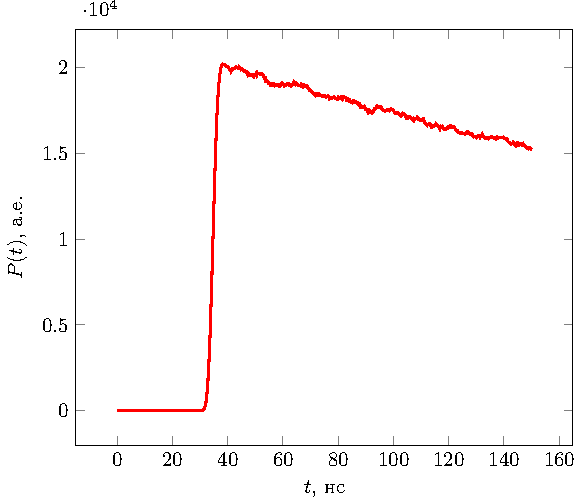
\includegraphics[scale=1]{fig/impuls.pdf}
    %\caption{Пример импульса для ретрекинга}
    %\label{fig:1}
%\end{figure}

\paragraph{Теоретическая основа.}%
\label{par:teoreticheskaia_osnova_}

Браун в своей работе вывел формулу, описывающего форму импульса в предположении
гауссовой плотности вероятности зеркальных площадок на морской поверхности.

\begin{equation}
    \label{eq:brown}
    P(t) = A e^{-v} (1 + \erf(u)), \text{ где}
\end{equation}
$u = \frac{t - \alpha \sigma_c^2}{\sqrt 2 \sigma_c}$, 
$v = \alpha(t - \frac{\alpha}{2} \sigma_c^2)$, 
в которых
$\alpha = \delta - \frac{\beta^2}{4} = 
\frac{4}{\gamma}\cdot \frac{c}{h} \qty(\cos 2\xi - \frac{\sin^2 2\xi}{\gamma})$
$A = A_0 \exp{\frac{- 4}{\gamma} \sin^2 \xi}$ и т.д (формула Брауна без изменений, не
хочется расписывать все обозначения целиком).

Одна из проблем данной формулы заключается в большом количестве коэффициентов,
а также в проблемах связанных с выбором начала отсчета времени. Эти факты могут
приводить к большим ошибкам даже при большом соотношении сигнал-шум.

\begin{figure}[h]
    \centering
    \includesvg{fig/imp}
    \caption{Качественная форма импульса с обозначением основных параметров.}
    \label{fig:impuls}
\end{figure}

Предлагается, использовать менее физичную, но более наглядную запись формулы
\eqref{eq:brown}:
\begin{equation}
    \label{eq:ice}
    P(t) = A \exp{ S_T (t - \frac{\tau}{2})} \qty(1 + \erf{\frac{t-
    \tau}{\sigma_L}}), \text{ где}
\end{equation}

$S_T$ -- коэффициент наклона заднего фронта импульса, 
 $\tau$ -- эпоха\footnote{ \sout{я не понял её определение, поэтому искал её
 исключительно численно, обходя её физический смысл} Пока писал раздел про
 калибровку времени разобрался зачем нужна эпоха и что это такое. }
$\sigma_L$ -- ширина переднего фронта импульса \footnote{Смысл $\sigma_L$ понятен из
формулы, однако у меня возникли вопросы с тем что считать шириной функции
ошибок и как найти этот коэффициент графически, потому для этого коэффициента
значение искалось в виде решения задачи оптимизации}.

\paragraph{Этап 1.Нахождение $S_T$.}%
\label{par:nakhozhdenie_s_t_}


Формула \eqref{eq:ice}, хороша тем, что можно найти некоторые коэффициенты, не
прибегая к задачам оптимизации. После прохождения пика импульса, функция ошибок
становится  медленно меняющейся функцией и можно записать равенство
\begin{equation}
    \label{eq:t>tmax}
    P(t) = 2A \exp{S_T (t - \frac{\tau}{2})}, \text{ при } t > t_{max},
\end{equation}
где $t_{max}$ -- ордината пика импульса.

Логарифмируя \eqref{eq:t>tmax}
\begin{equation}
    \ln P(t) = \ln 2A + S_T( t - \frac{\tau}{2}) = S_T t + \const 
\end{equation}
мы получаем линейную функцию времени. Значит, построив логарифм формы импульса при
$t>t_{max}$ и найдя коэффициент наклона получившейся прямой мы можем найти
наклон заднего фронта $S_T$. Подобная процедура проведена на рис.\ref{fig:S_T}
 \begin{figure}[h]
    \centering
    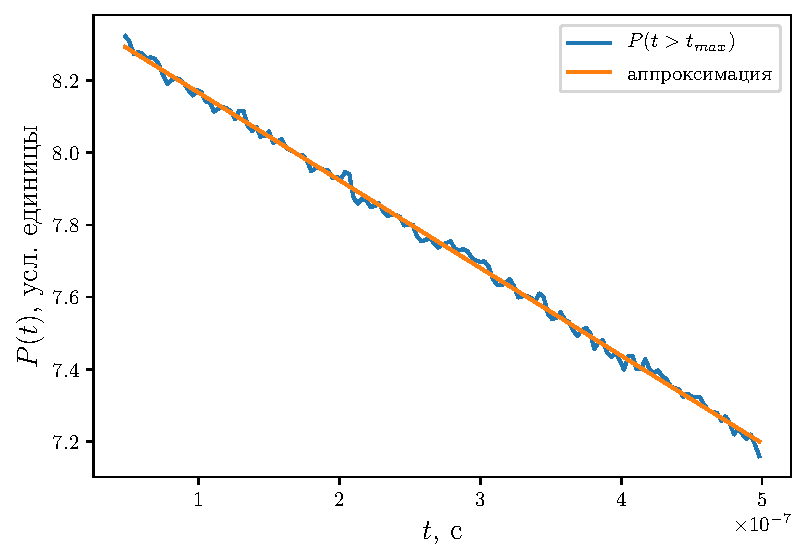
\includegraphics[width=\linewidth]{../project/radiolocator/imp08_7_1.pdf}
    \caption{Нахождение наклона заднего фронта}
    \label{fig:S_T}
\end{figure}

\paragraph{Этап 2. Нахождение $\sigma_L$}%
Как видно из рис.\ref{fig:erf}, при $t<t_{max}$ функция ошибок ведет себя
быстрее экспоненты, а значит можно написать приближенное равенство
\begin{equation}
    \label{eq:erf}
    P(t) \approx A \qty(1 + \erf{\frac{t - \tau}{\sigma_L}})
\end{equation}

\begin{figure}[h]
    \centering
    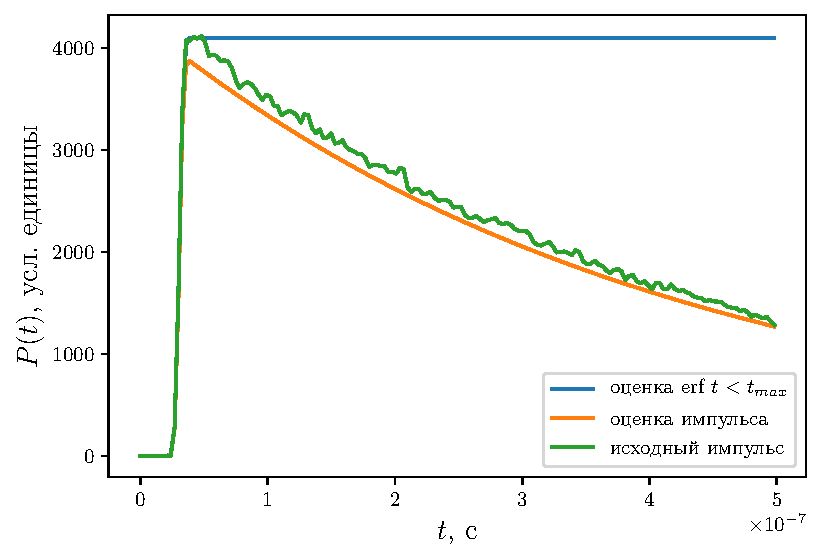
\includegraphics[width=\linewidth]{../project/radiolocator/imp08_7_2.pdf}
    \label{fig:erf}
\end{figure}

Аппроксимируя импульс при $t<t_{max}$ формулой \eqref{eq:erf} мы получим оценку
коэффициентов $A,~\tau,~\sigma_L$. При этом, интересовать нас на этом этапе
будут в основном  эпоха $\tau$ и ширина переднего фронта  $\sigma_L$.

\paragraph{Этап 3. Выравнивание по времени.}%
\label{par:etap_3_vyravnivanie_po_vremeni_}

Пока я писал этот этап и строил графики для него, то обнаружил, что
необходимости в калибровке времени у меня на самом деле нет. Всё благодаря
формуле ICE, которая вводит дополнительный независимый параметр $\tau$, который
и будет двигать положение максимума при решении задач оптимизации. 

В формуле Брауна же положение максимума зависит от коэффициентов, $\alpha$ и
$\sigma_c$, что жестко привязывает функцию к значениям времени. 
\sout{На практике импульс по оси времени располагается не так, как того требует
формула Брауна. Это связано с разным выбором начала времени отсчета $t$. }

\sout{Чтобы избавить наш метод от зависимости от абсолютного значение времени и
<<научить>> его сравнивать, разнесенные во времени теоретический и практический
импульс (см. рис. \ref{fig:deltat}), нужен этот этап. }

\sout{После первых двух этапов алгоритма, у нас есть все оценки коэффициентов для
формулы \eqref{eq:ice}. Дифференцируя формулу \eqref{eq:ice} не сложно получить
выражание для координаты максимума импульса, но я искал его численно, поскольку
эта операция не отнимает много времени.}

\sout{Зная теперь положения максимума по формуле \eqref{eq:ice}, мы можем выполнить
преобразование координат и сместить максимум практического импульса, на то
место, где он должен быть согласно теории (см. рис.\ref{fig:deltat1}).}

\paragraph{Этап 4. Заключительная аппроксимация.}%
\label{par:etap_4_zakliuchitel_naia_approksimatsiia_}

\sout{Откалибровав ось времени и}  Имея оценки параметров аппроксимации по различным
участкам функции $P(t)$ мы можем использовать формулу  \eqref{eq:ice} для всего
импульса целиком.

То есть, теперь нам необходимо решить задачу оптимизации параметров для функции 
\begin{equation}
    \label{eq:ice}
    P(t) = A \exp{ S_T (t - \frac{\tau}{2})} \qty(1 + \erf{\frac{t-
    \tau}{\sigma_L}})
\end{equation}
с начальными условиями для параметров $A, S_T, \tau, \sigma_L$, полученных на
предыдущих этапах\footnote{ Я тестировал этот спобоб для разных импульсов и
пришел к выводу, что на этом этапе варьировать $S_T$,  $\tau$,  $\sigma_L$
достаточно лишь на несколько процентов, поскольку предыдущие этапы с хорошей
точностью дали оценку параметров. В основном, этот этап необходим для
калибровки амплитуды.}. 


На рисунках ниже продемострированы результаты работы этого алгоритма на
различных формах импульса (меняются углы отклонения антенны).

\begin{figure}[H]
    \centering
    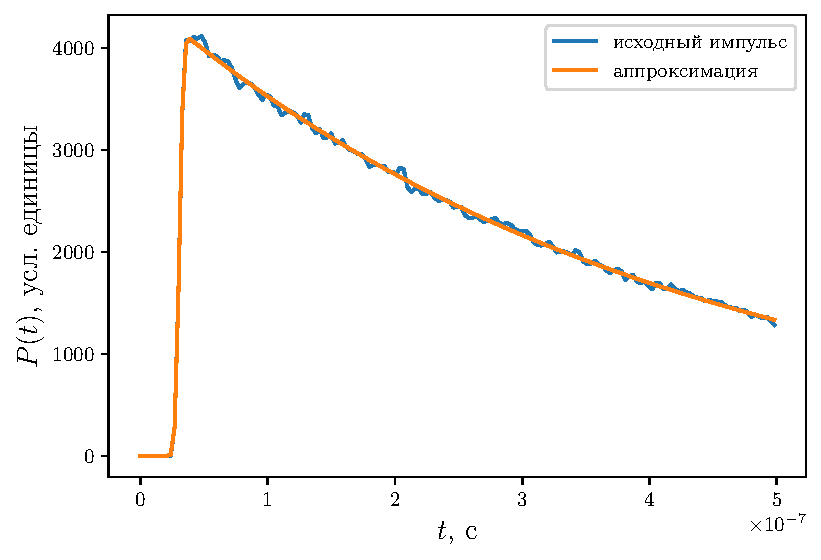
\includegraphics[width=\linewidth]{../project/radiolocator/imp08_7_3.pdf}
    \caption{Обработка файла imp08\_7.dat}
    \label{fig:ex}
\end{figure}


\begin{figure}[H]
    \centering
    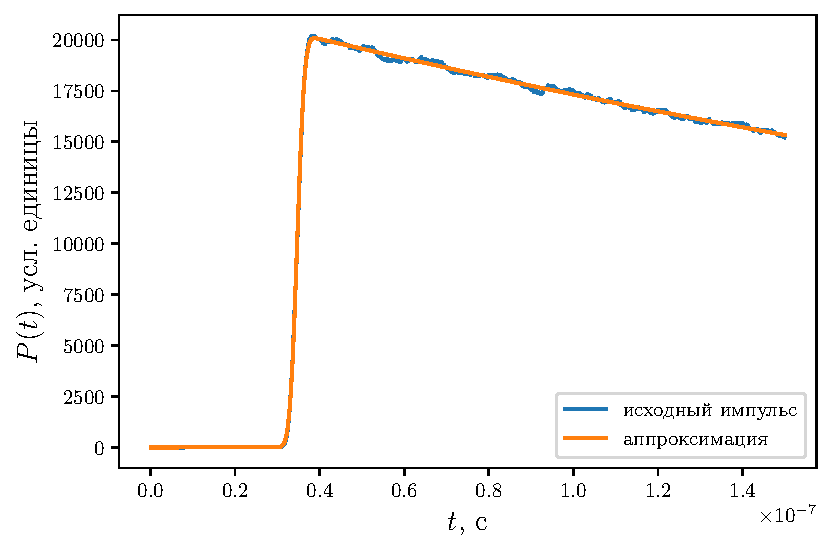
\includegraphics[width=\linewidth]{../project/radiolocator/imp_5_3.pdf}
    \caption{Обработка файла imp\_5.dat}
    \label{fig:ex}
\end{figure}


\begin{figure}[H]
    \centering
    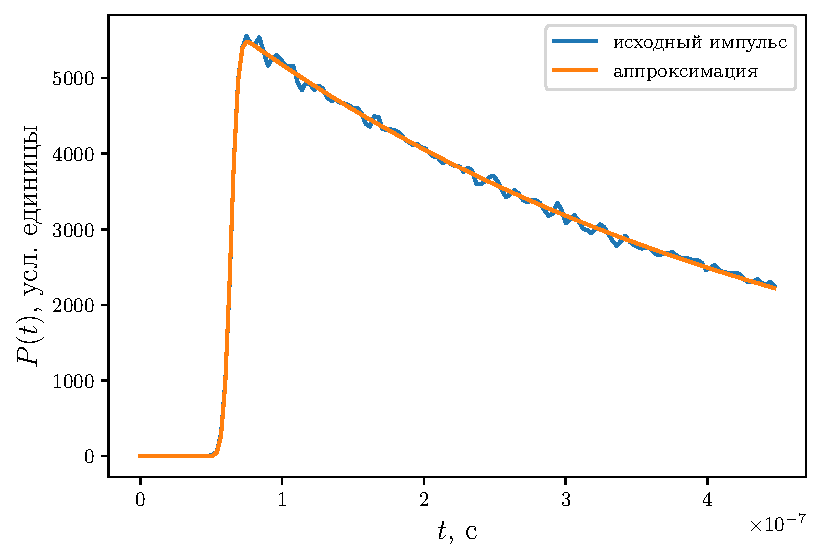
\includegraphics[width=\linewidth]{../project/radiolocator/imp04_10_3.pdf}
    \caption{Обработка файла imp04\_10.dat}
    \label{fig:ex}
\end{figure}


\begin{figure}[H]
    \centering
    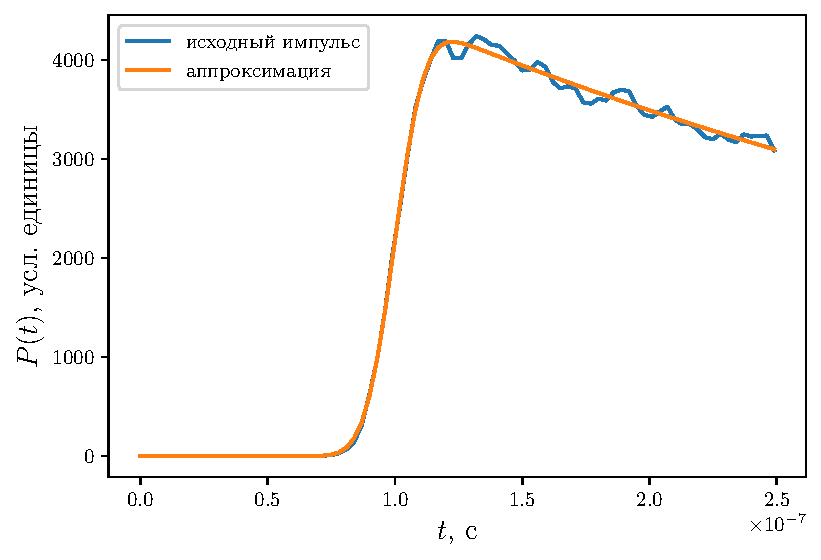
\includegraphics[width=\linewidth]{../project/radiolocator/imp_15a_3}
    \caption{Обработка файла imp15a.dat}
    \label{fig:ex}
\end{figure}




\paragraph{Этап 5. Восстановление параметров. На стадии планирования. В тексте
есть вопросы.}%
\label{par:etap_5_vosstanovlenie_parametrov_}

Не сложно найти связь коэффициентов в формуле Брауна \eqref{eq:brown} и формуле
ICE  \eqref{eq:ice}:

\begin{gather}
    \label{eq:}
    S_T = - \alpha\\
    %\tau = \alpha \cdot \sigma_c^2 \\
    \sigma_l = \sqrt 2 \sigma_c
\end{gather}

Найдя коэффициенты для формулы \eqref{eq:ice} перейдем к формуле \eqref{eq:ice}
и будем решать систему коэффициентов относительно неизвестных параметров
радиовысотомера и состояния морской поверхности.

\begin{gather}
    A(A_0,\xi) = A_0 \exp{-\frac{4}{\gamma} \sin^2 \xi} \\
    \alpha(\xi,h) = \frac{4c}{\gamma h} \cdot (\cos 2\xi - 
            \frac{\sin^2 2\xi}{\gamma}) \\
    \sigma_c^2 = \sigma_p^2 + \sigma_s^2
\end{gather}


Основной вопрос заключается в нахождении $\xi$ и $h$.
Для трех неизвестных параметров $A_0$,  $\xi$,  $h$ у меня имеются только два
уравнения.  Можно ли найти высоту, на
которой находится спутник, зная время между испусканием сигнала и его приемом
или такая задача слишком сложная? 
Альтернативно, могу ограничить диапазон изменения $\xi$ и решить эту
незамкнутую систему уравнений численно. Однако тогда высота и отклонение будут
определяться неоднозначно. 



\bibliography{diplom}
